\chapter{Appendix \autoref{chap:understanding}}


\section{Implementation details for the experiments}
\label{app:understanding:empirical}

\begin{table}[]
    \centering
    \begin{tabular}{c|c|c}
        Parameter & MinAtar & DMC \\\hline 
        Initial steps (Random policy) & $5000$ & $5000$  \\
        Env steps per update step & $4$ & $1$\\
        Batch size & $512$ & $512$\\
        Exploration $\epsilon$ & $0.05$ & $0.01$\\
        RL learning rate & $0.0003$ & $0.0003$\\
        Model/decoder learning rate & $0.0003$ & $0.0003$\\
        Encoder learning rate & $0.0001$ & $0.0001$\\
        Target network update interval & $1000$ & n/a\\
        Soft update $\tau$ & n/a & $0.995$ \\
        Discount factor $\gamma$ & $0.99$ & $0.99$\\
        Model forward prediction steps & $4$ & $4$\\
    \end{tabular}
    \caption{Hyper-parameters the RL experiments}
    \label{tab:hyper_minatar}
\end{table}

For the Minatar experiments, we use a simple Double DQN architecture \parencite{van2016deep}.
We find that our implementation performs roughly on par with those reported by \textcite{young19minatar}, however we changed the network architecture slightly to allow a clear "encoder" and "prediction head" split.

We implement the latent self-prediction loss using a periodically updated copy of the encoder network. This hard update of the encoder target is synchronized with the Q target network update.

Our networks are parameterized as presented in \autoref{tab:net_minatar}

\begin{table}
\begin{center}
\begin{tabular}{c|c|c}
     & ConvLayer & channels=$16$, kernel=$(3,3)$, padding=$0$, stride=$(1,1)$ \\
     Encoder $\Phi$ & ELU activation & -- \\
     & Dense Layer & out\_size=$100$\\
     & ELU activation & -- \\\hline
     & Dense Layer & out\_size=$256$ \\
     Latent Model $F$ & ELU activation & -- \\
     & Dense Layer & out\_size=$100$\\\hline
     & Dense Layer & out\_size=$10\cdot10\cdot16$\\
     Decoder $\Psi$ & ELU activation & -- \\
     & ConvTranspose Layer & kernel=$(3,3)$, padding=$1$,  stride=$(1,1)$\\\hline
     & Dense Layer & out\_size=$256$ \\
     Q head $\hat{V}$ & ELU activation & --\\
     & Dense Layer & out\_size=action\_space
\end{tabular}
\end{center}
\caption{Network architecture for the MinAtar experiments.}
\label{tab:net_minatar}
\end{table}

Relevant hyper-parameters are shown in \autoref{tab:hyper_minatar}.

The random noise matrix is sampled from a Bernoulli distribution with $p(1) = 0.1$.
The distortion matrix was created using a random matrix of size $10\cdot10\cdot\mathrm{channels} \times 10\cdot10\cdot\mathrm{channels}$ with entries independently sampled from a Bernoulli distribution with $p(1) = 0.2$. 
This was chosen to have a similar sparsity in the distraction as in the main observation channels.
Additionally, we verified that the matrix was invertible and $\lVert \gO \rVert_1 < 255$ to ensure that the replay buffer implementation would not overflow.


The DMC results were obtained using the TD3 algorithm \parencite{td3} with constant Gaussian noise with standard deviation of $0.01$ added for exploration following \textcite{yarats2021image}. In addition to the Q function network, TD3 also requires an actor network. We do not propagate any gradients from the actor network into the encoder, following standard practice in actor-critic learning.

Networks for the DMC implementation are shown in \autoref{tab:net_mujoco}.

\begin{table}
\begin{center}
\begin{tabular}{c|c|c}
     & Dense Layer & out\_size=$256$ \\
     Encoder $\Phi$ & ELU activation & -- \\
     & Dense Layer & out\_size=$256$\\
     & ELU activation & -- \\\hline
     & Dense Layer & out\_size=$256$ \\
     Latent Model $F$ & ELU activation & -- \\
     & Dense Layer & out\_size=$100$\\\hline
     & Dense Layer & out\_size=$10\cdot10\cdot16$\\
     Decoder $\Psi$ & ELU activation & -- \\
     & Dense Layer & out\_size=obs\_dim\\\hline
     & Dense Layer & out\_size=$256$ \\
     Q head $\hat{V}$ & ELU activation & --\\
     & Dense Layer & out\_size=1\\\hline
     & Dense Layer & out\_size=$256$ \\
     Actor head & ELU activation & --\\
     & Dense Layer & out\_size=action\_dim
\end{tabular}
\end{center}
\caption{Network architecture for the DMC experiments.}
\label{tab:net_mujoco}
\end{table}
In the DMC experiments, we used isotropic Gaussian noise for the distracting noise, and a copy of the \emph{humanoid} environment as the distraction.

Full code is available at \url{https://github.com/adaptive-agents-lab/understading_auxilliary_tasks}.


\section{DMC results}
\label{app:understanding:mujoco_results}

The DMC environments have a very different observation structure and transition dynamics compared to those of the MinAtar games. The observation spaces are dense and often contain topological discontinuities such as those outlined in \autoref{app:observation_motivation}.

All experiments are repeated across 10 seeds.

We find slightly different results in these environments compared to MinAtar, especially about the efficacy of the latent self-prediction and observation reconstructions in the stand-alone setting (\autoref{fig:muj_sta} and \autoref{fig:muj_sta_rew}). Overall, latent self-prediction performs much more strongly in these environments compared to the MinAtar experiments, especially when using it as a stand-alone loss.
Curiously, in the only environment where observation prediction shines (quadruped-walk), stand-alone latent self-prediction and reward prediction seems to outperform all other test settings.
This highlights the second important difference between the MinAtar games and the DMC suite: dense rewards.
We conjecture that most of the differences between observation prediction and latent self-prediction in the DMC suite comes from dense rewards and different topological continuity, but a precise investigation is needed in future work.

Finally, our assumptions about the impact of noise distortions on the efficacy of different loss functions seems to be much more clearly apparent in DMC than in MinAtar. This suggests that the differing primary observation spaces also change how the learning process interacts with the noise, i.e. because the spectral properties of the underlying environments might differ.
Especially in the challenging distraction setting of structured noise, non trivial policies (as measured by a strong performance improvement over a random baseline) can only be observed in 7 out of the 15 environments. Of these 7, latent self prediction seems to outperform the other baselines in 3 cases, only falling behind in 1. However, we observed that the pendulum environment has a strong bimodal distribution with some runs completely failing to perform for each experimental scenario, so the number of seeds might be insufficient to disambiguate performance here, as evidenced by the large confidence interval at the $95\%$ level.

Overall, 10 seeds, even though widely used in the community, might not be sufficient to fully represent the performance in the DMC suite, suggesting that more work is needed on the inherent variations of these environments.
We do not present aggregate performance over the environments, as the different reward scales makes a comparison prone to be driven by outliers such as the humanoid environments, in which several algorithms fail to learn at all at 10 seeds.

\begin{figure}
    \centering
    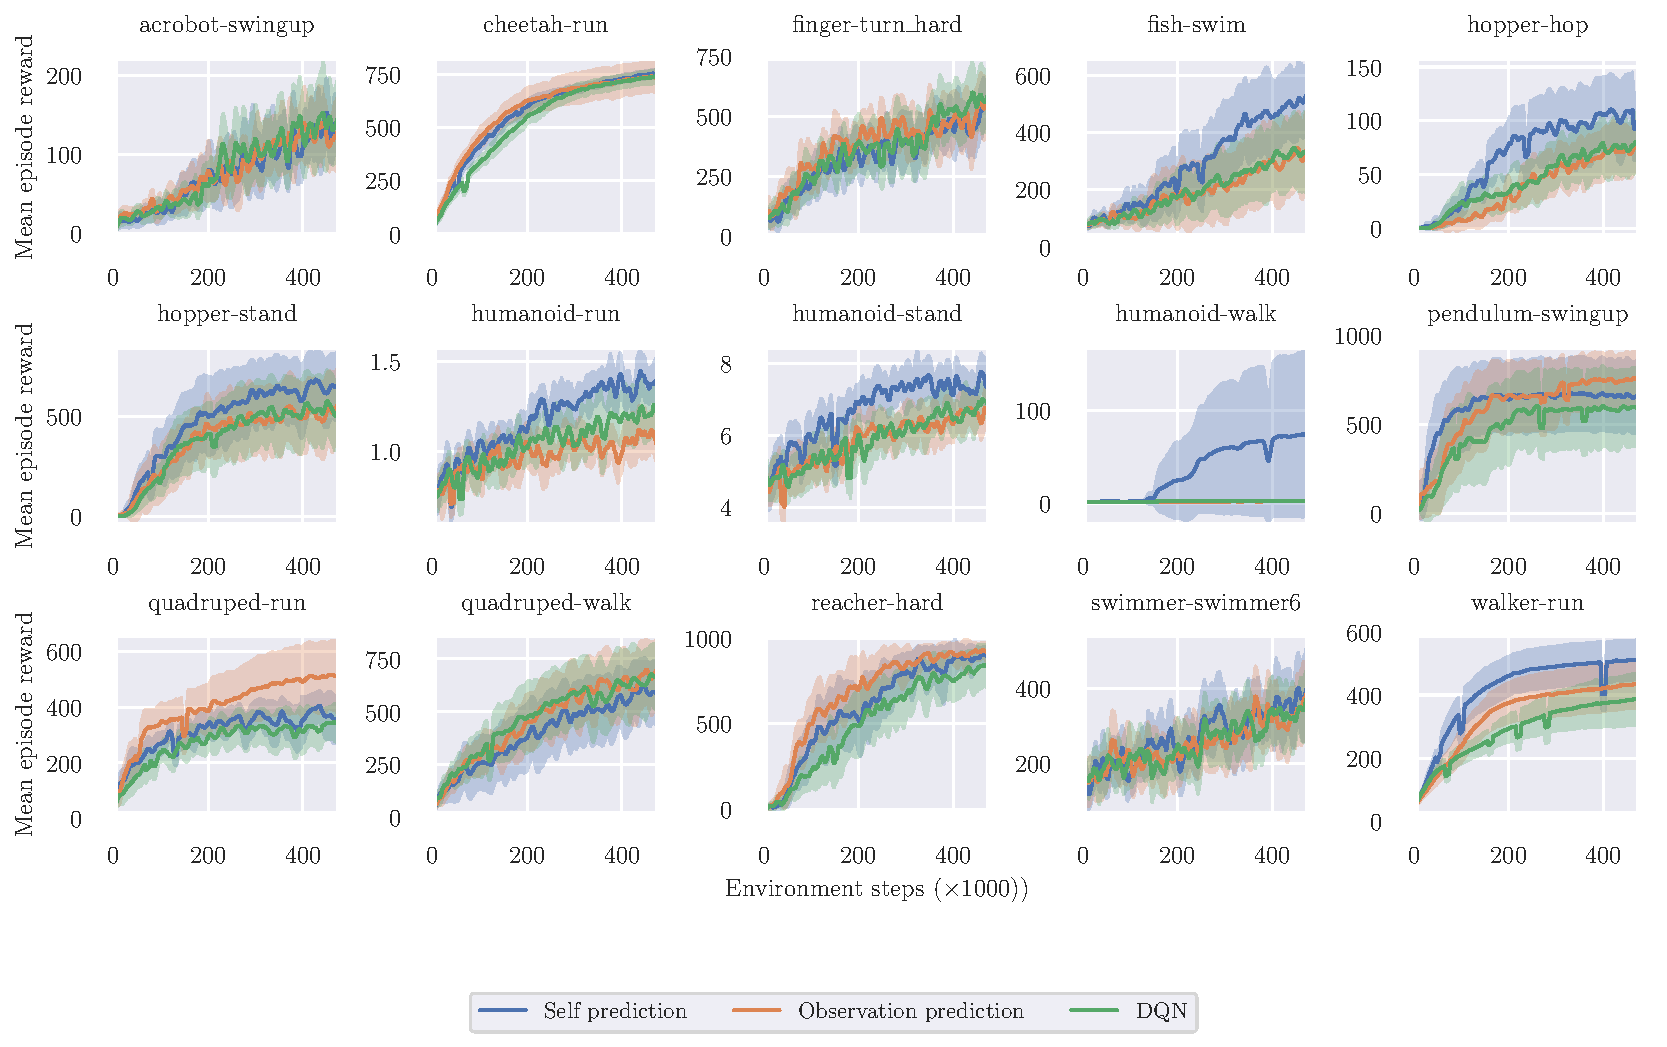
\includegraphics[width=\textwidth]{figures/understanding/rlc2024_mujoco.pdf}
    \caption{DMC: Auxiliary task scenario}
    \label{fig:muj_aux}
\end{figure}

\begin{figure}
    \centering
    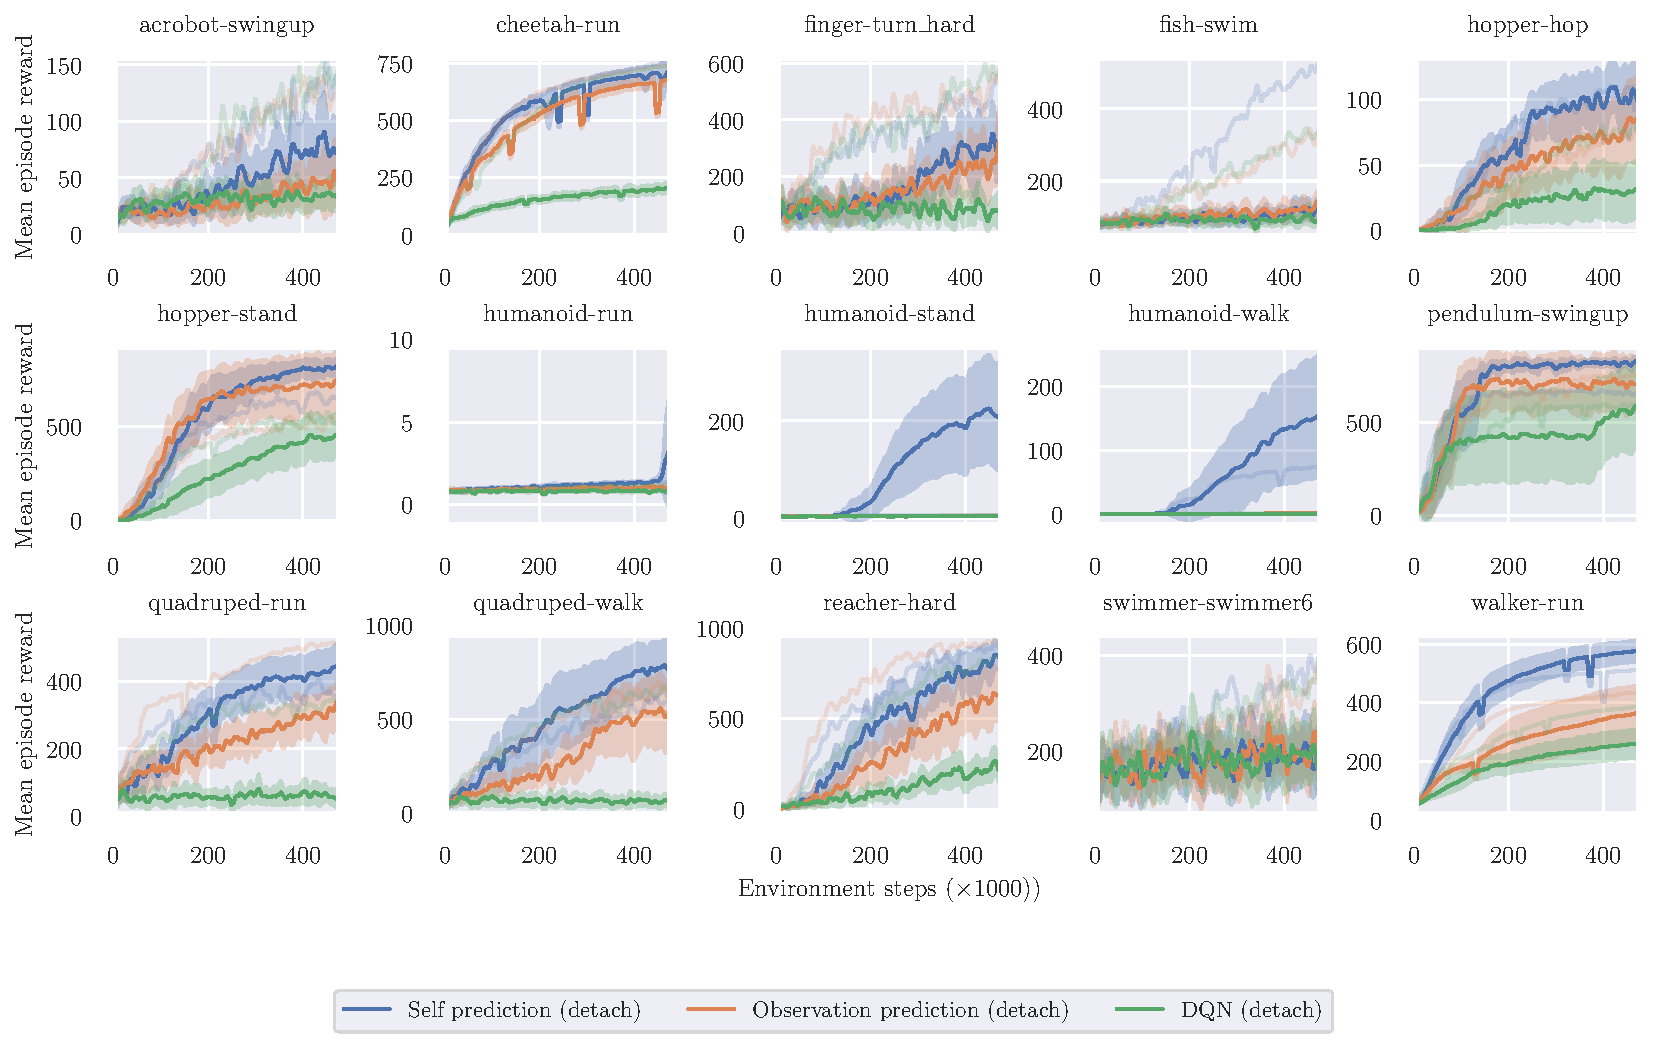
\includegraphics[width=\textwidth]{figures/understanding/rlc2024-detach_mujoco.pdf}
    \caption{DMC: Stand alone scenario}
    \label{fig:muj_sta}
\end{figure}

\begin{figure}
    \centering
    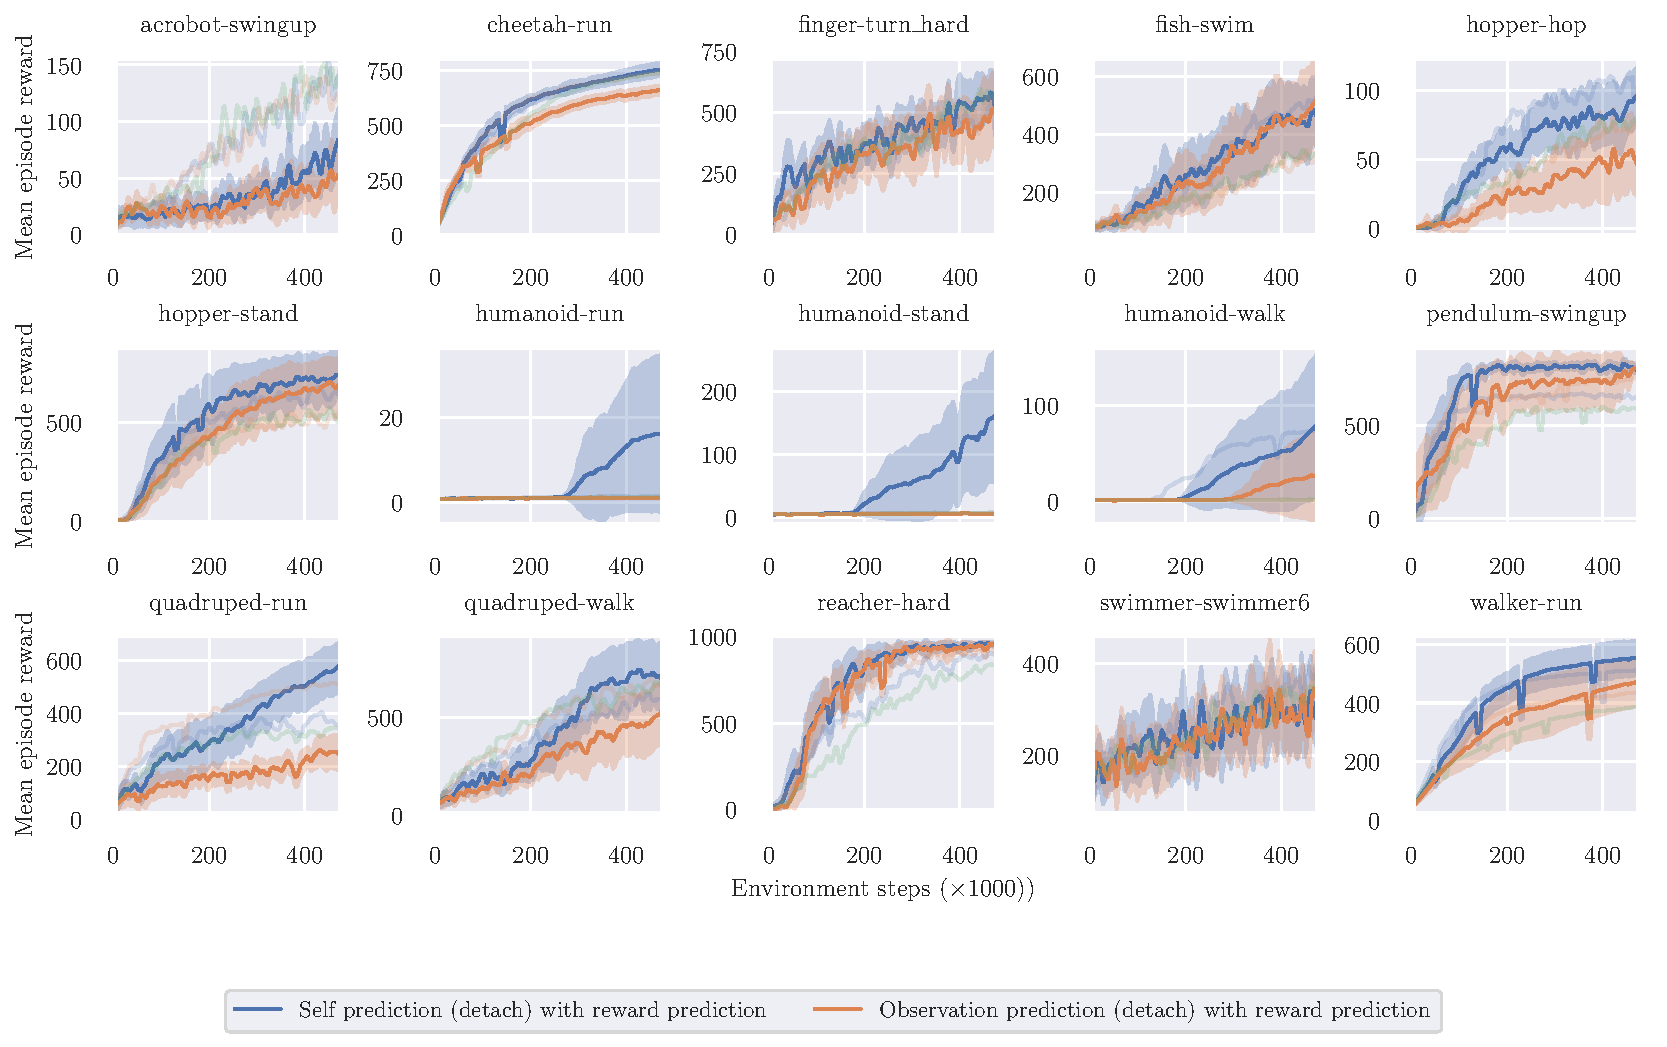
\includegraphics[width=\textwidth]{figures/understanding/rlc2024-rew-detach_mujoco.pdf}
    \caption{DMC: Auxiliary loss + reward prediction, not TD}
    \label{fig:muj_sta_rew}
\end{figure}

\begin{figure}
    \centering
    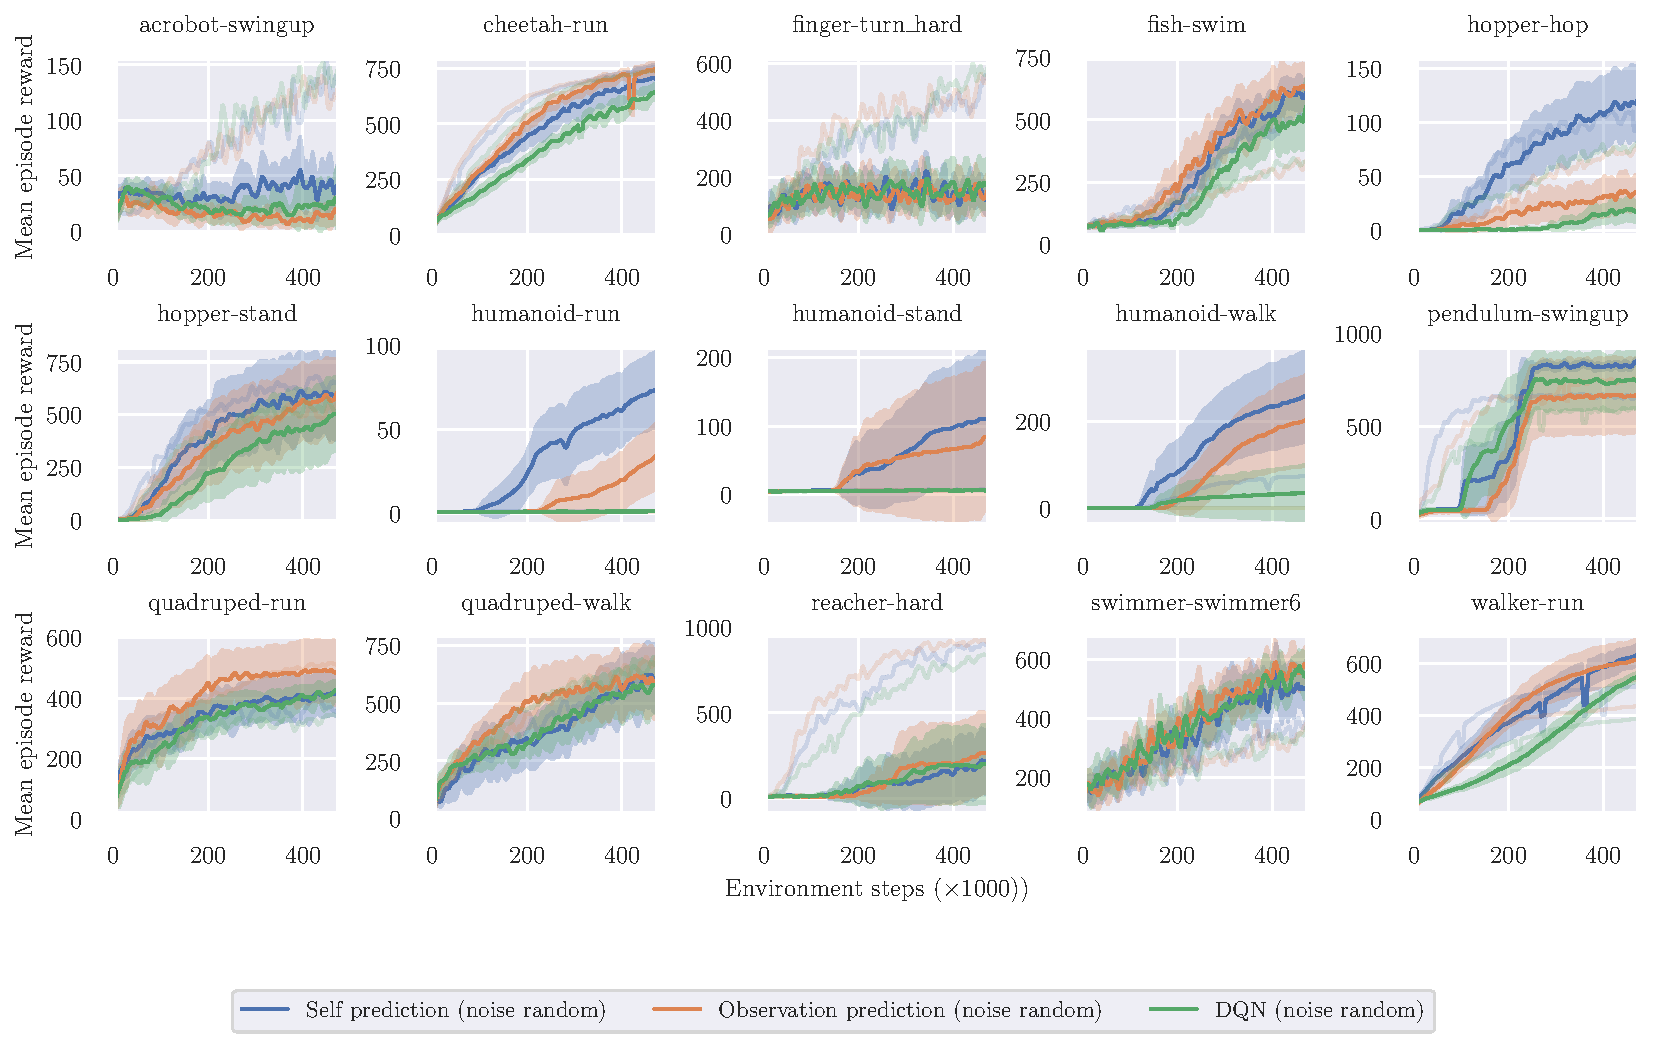
\includegraphics[width=\textwidth]{figures/understanding/rlc2024-random-noise_mujoco.pdf}
    \caption{DMC: Random noise distraction}
    \label{fig:muj_ran_noi}
\end{figure}

\begin{figure}
    \centering
    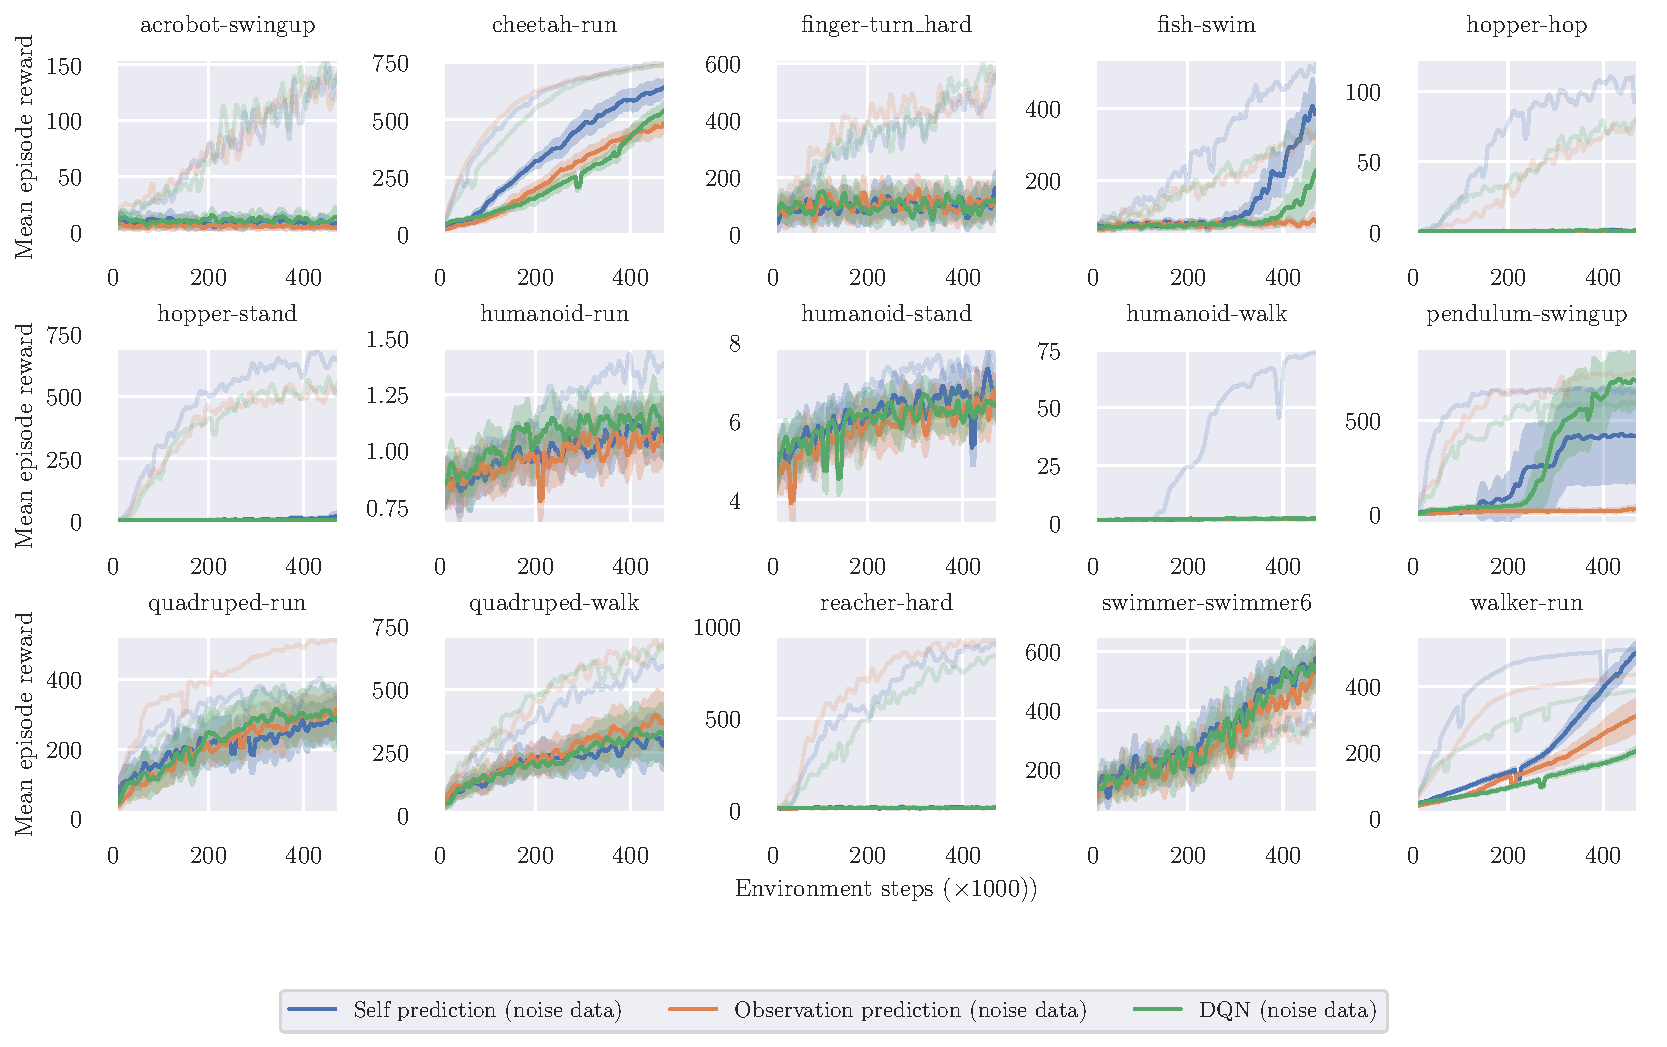
\includegraphics[width=\textwidth]{figures/understanding/rlc2024-random-data_mujoco.pdf}
    \caption{DMC: Structured distraction}
    \label{fig:muj_ran_str}
\end{figure}

\begin{figure}
    \centering
    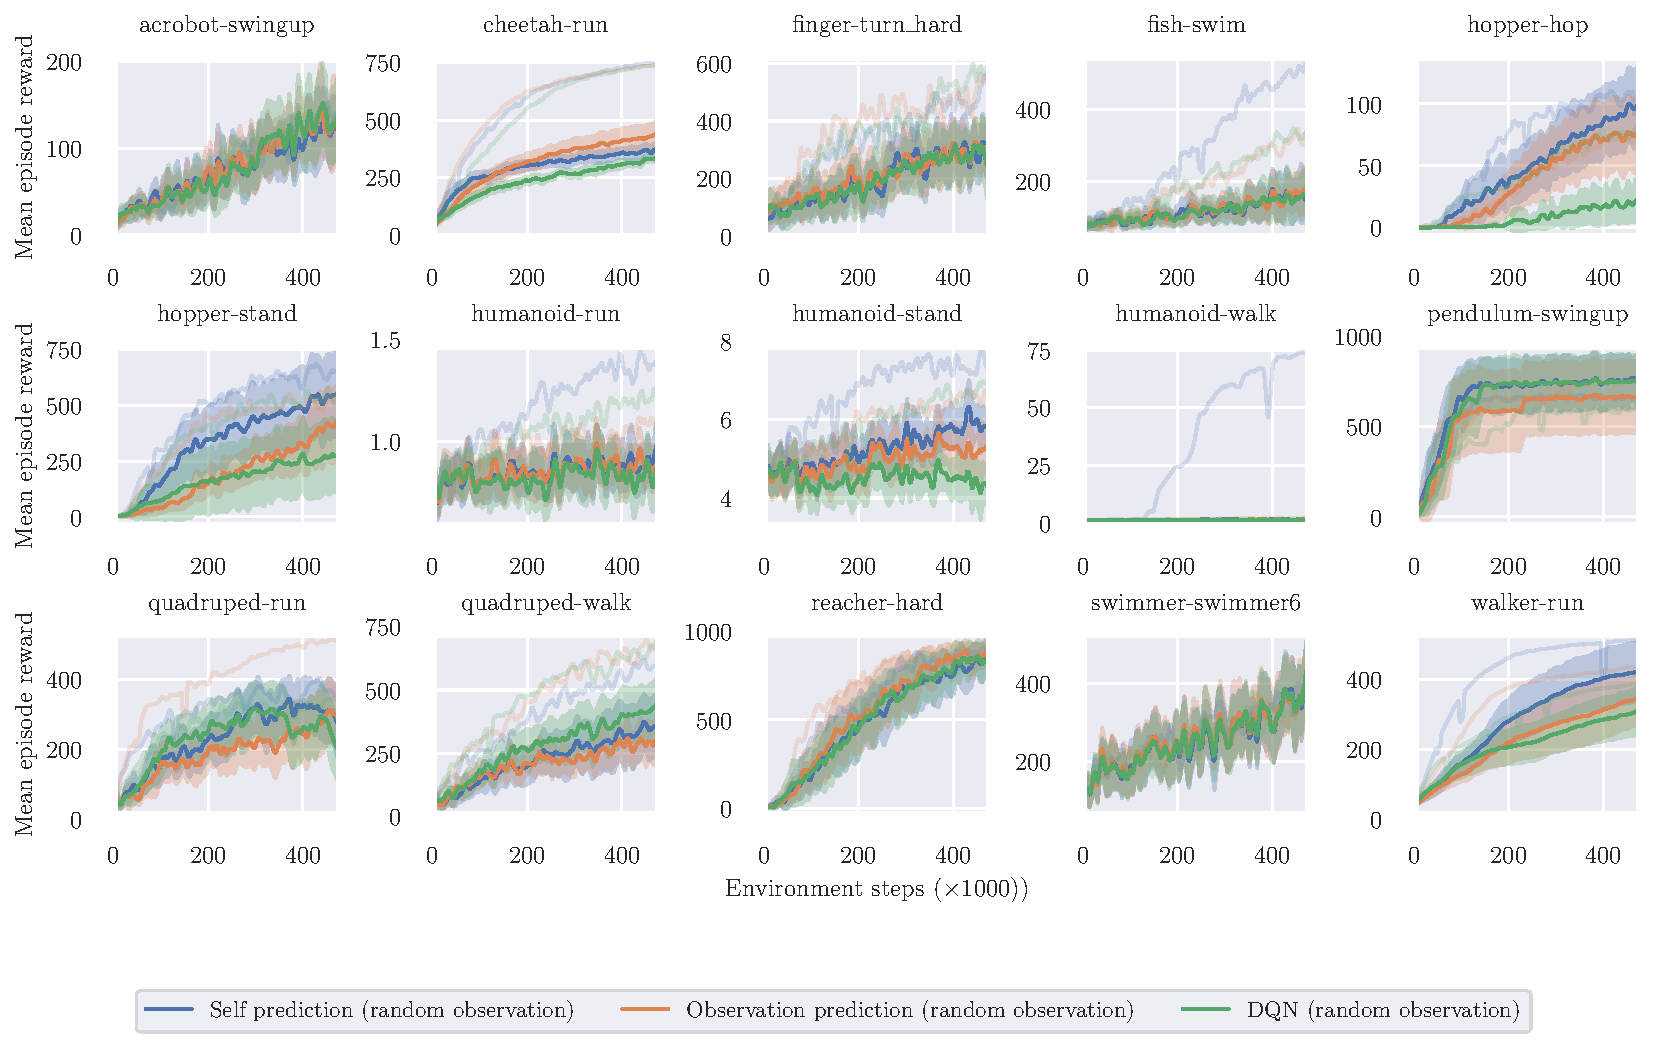
\includegraphics[width=\textwidth]{figures/understanding/rlc2024-distorted-fixed_mujoco.pdf}
    \caption{DMC: Observation space distortion}
    \label{fig:muj_dis}
\end{figure}


\section{Limitations}
\label{app:limitations}

While our paper aims to minimize the theory-practice gap with careful experimentation, we nonetheless need to make several assumptions that are both limitations and also potential for additional analysis in future work.
As our aim is to make theory useful and accessible for practitioners, we aim to be very open and clear about our limitations here.

\textbf{Limitations of the analytical framework:} From previous work \parencite{tang2022understanding,lelan2023bootstrapped} we inherit the limitation of studying deterministic models in potentially stochastic environments.
This is a necessary limitation, as considering the stochastic equivalents of e.g. the observation prediction loss would render the model and their gradients non-linear due to the introduction of a softmax or similar constraint.
As other works carry the same limitation, we believe that this does not render our work inapplicable, but it does suggest the need for more powerful mathematical tools in future work.

We also conduct all of our theoretical work in the on-policy policy evaluation regime, while our empirical study includes both off-policy policy estimation and policy improvement.
Again, this is a limitation inherited from all related work.
As our theoretical predictions are still validated, we consider this an acceptable limitation, but studying the impact of off-policy samples and shifting policies is an important step for future work.

\textbf{Limitations of the formalism:} Our notion of observation distortion requires unnaturally large observation spaces. Again, this stems from our adherence to a linear framework.
While the observation space of e.g. the MinAtar games is relatively large, depending on the game a 300-1000 dimensional vector, this is still substantially smaller than the total number of states.
Studying these kinds of nonlinear image transformations in more detail would require deviating farther from the previous literature.

In this paper, we aim to (re-)introduce the notion of distraction into the learning dynamics literature, and so we use a relatively simplistic notion of distraction.
Going beyond the independence assumption in the distraction model (due to the Kronecker formulation) and analyzing more complex forms of distractions e.g. processes in which the reward-relevant process causally influences the distracting process but not vice versa is an exciting direction for future work.
